\documentclass{standalone}

\begin{document}

\section[SymptomsNet]{SymptomsNet}\label{chimera:symptomsnet}

Find relationships between symptoms and diseases and their reflections on system-wise perspectives such as genomics and metabolomics still remains a crucial issue for medical research but nonetheless an open one.
The relation between symptoms and diseases can be used to see analogies and co-occurrences of different pathologies, including morbidity and co-morbidity.
The construction of a unique and consistent database of these kind of data is an open problem for the research and a crucial task for many actual projects.
The main problems arise from the complexity and heterogeneity of the available data and from the many nomenclatures used by different public databases.
In fact, in many cases it is not so clear how to infer about the association between symptoms and diseases, and, in addition, different data sources provide different associations.
These information are stored as sentences and periods, of variable length and we have to face on the problem of the different synonyms and periphrases used to describe the same concept.

In our work we used large-scale public on-line databases to construct a bipartite network of human symptoms-diseases.
A bipartite network (or \emph{bigraph}) is a graph whose nodes can be divided into two disjoint and independent sets: the underlying adjacent matrix is rectangular and it describes the connections between the $N$ elements of the first set and the $M$ elements of the second one.
We can always lead back to a square matrix $(N\cdot M \times N\cdot M)$ using zero blocks for the intra-group connections.
We used common tools of natural language processing to clean and standardize the data to maximize the overlap between the different sources.
After its construction, this network is used to establish a score for the different words based on the centrality measure of the node.
This complex map of association can further be used to connect other data sources and enrich the diseases description from other medical points-of-view.

Many on-line databases offer auto-diagnosis tools and search engine in which the user can insert a list of symptoms or diseases and obtain the corresponding \quotes{diagnoses}.
While many international databases are quite consistent and supported by medical/biological research groups, the available data in Italian language are quite scarce.

Using the Italian version of the few public \emph{on-line doctor} websites found we obtained the needed information.
We applied a set of custom web scraping pipelines to different web pages to extract the medical information and we mainly focused on sites which highlight the relationships between symptoms and diseases.
We would stress that the extremely variety of the websites requires an equally varied set of web-scraping algorithms.
Thus for each web page taken into account a relative web-scraper was developed.
As discussed above the Italian data sources are quite fewer than the English ones so only three web pages were involved into our analysis: \href{https://m.my-personaltrainer.it/}{My PersonalTrainer}\footnote{
  Arnoldo Mondadori Editore S.p.A.
}, \href{http://www.sanihelp.it/}{SaniHelp}\footnote{
  Terms and conditions available \href{https://www.iubenda.com/terms-and-conditions/210132}{here}.
} and \href{http://www.sapere.it/}{Sapere.it}\footnote{
  De Agostini Group.
}.
All these three sites provide an organized series of tables which associate a disease to the corresponding symptoms and thus are easily to treat with web-scraping algorithms.
These databases are not reliable from a scientific point-of-view and their vulnerability is shown also by a non-rigid labeling of the two classes: in multiple cases we can find a disease as symptom of a different one and in many cases there is not a perfect agreement between the three data sources.
Possible issues related to an incorrect disease information could not be attributed to our \textsf{web-scraping} pipeline, but they should be already present into the original data which, we want remark it, they are the only Italian datasets public available and found.

The data extracted from the three websites cover a wide range of possible diseases and from each of them we obtained a network with a size of few thousand of nodes, our \textsf{SymptomsNet}.
The overlap of the single words contained in the \quotes{disease-sentences} is quite low so a robust pre-processing was needed.
The nodes were processed by standard natural language processing techniques and from each name the word stem was extracted to maximize the merging between the sources.
If two diseases show different symptoms we decided to concatenate the list of edges to not lose information.

The processed outputs generated a network with \numprint{2285} nodes and more than 29k links (only the 1\% of the total number of possible links).
The final \textsf{SymptomsNet} obtained by the merging of the three database sources is reported in Fig.\ref{fig:net} in which the node sizes are proportional to the number of their connections (Tab.\ref{tab:rank} for the top ranking links).

\begin{figure}[htbp]
\centering
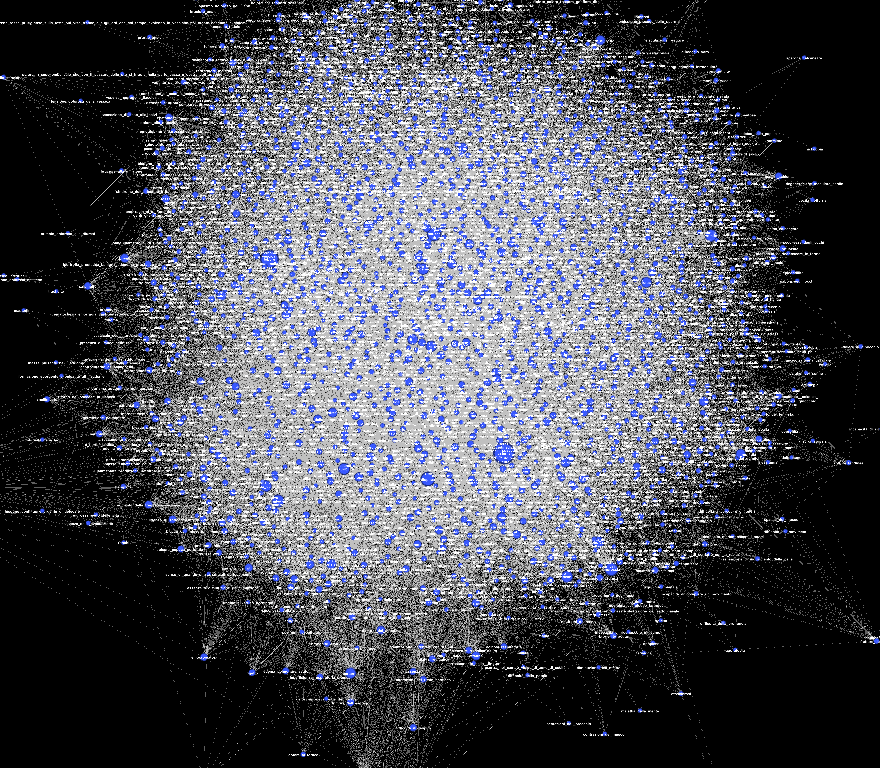
\includegraphics[width=.8\linewidth]{symnet.png}
\caption{Symptoms-disease network generated by the merging of three public Italian web-pages of auto-diagnosis search engine.
The network connects symptom and disease words according to validation agencies.
The network comprise \numprint{2285} nodes and more than 29k links.
The node sizes are proportional to their centrality (number of connections or degree score).
In this way the most common symptoms/diseases represent the biggest nodes.
}
\label{fig:net}
\end{figure}

\begin{table}[htbp]
\centering
\begin{tabular}{lccc}
\hline \rowcolor{darkgrayrow}
Disease/Symptom & degree \\
\hline
Astenia         & 384    \\
Febbre          & 313    \\
Dispnea         & 225    \\
Nausea          & 222    \\
Anoressia       & 201    \\
Ematemesi       & 193    \\
Vomito          & 182    \\
Debolezza       & 176    \\
Affaticamento   & 176    \\
Esaurimento     & 172    \\
Mancanza Forze  & 168    \\
Edema           & 158    \\
\hline
\end{tabular}
\caption{Top ranking links in the \textsf{SymptomsNet}. We can notice \quotes{periphrases/synonyms} associated to the same symptom as \emph{Debolezza} and \emph{Mancanza Forze} which are left to increase the samples heterogeneity for the synthetic text generator.}
\label{tab:rank}
\end{table}

In this simple example we can already notice as the most central (big) nodes are associated to the most common symptoms-diseases, as expected.
This result can be already interpreted as a validation of the performed processing.
We can notice from Tab.\ref{tab:rank} that also in the top ranking nodes we find some diseases and related synonyms: this could be an issue for the network structure since it means that the developed pipeline of processing is not able to merge together different words with equal meaning.
However, the project purposes was to create a reasonably good diseases ontology and this issue could be turned to a strength of our applications since it proves that we have an agreement between the different databases (synonyms have comparable degree score and thus same importance) and it highlights the variety of mined terms (different names which identify the same disease).
In fact, this kind of occurrences allow to consider a wide range of possible synonyms in the scorer attribution and so they can enforce the text analyses required by the FiloBlu project: the node degree can be used as weight (1/degree) for text words and thus we can obtain a simple score for the message given by the sum of the mapped keywords.

We conclude that from this very simple and preliminary work we are able to propose a novel symptoms-disease network based on Italian public databases and far as the author knows no other equivalent results are reported in literature.
This work allowed also the realization of a novel database obtained by the union of public available data.
The extracted centrality measures can be used as weights for the corresponding symptoms/diseases and a valid input to model the word frequency/importance in text analyses.

The developed network is based on a bipartite graph which associates disease nodes to symptom ones.
These results highlight the potentiality of such structures and they brought us to further investigate about them and their creation.
In particular, reiterating the same procedure we could be able to join together different bipartite graphs and obtain a network-of-networks structure which store multiple type of information.
This is the main idea behind the \textsf{CHIMeRA} project.
To this purpose we have to manage more reliable data sources and improve our natural language processing pipeline to increase the datasets overlap and minimize the amount of synonyms.
All these tasks can be easier performed using English words and validated databases.
In the next sections we are going to discuss about what natural language processing means in modern researches and we will describe the pipeline and databases used in the development of the \textsf{CHIMeRA} network.

\end{document}
